\documentclass{beamer}% {{{
\usepackage{amssymb, latexsym, amsmath, graphics, fullpage, epsfig, amsthm, relsize, pgf, tikz, amsfonts, makeidx, latexsym, ifthen, hyperref, calc}
%\usepackage{eucal} this is a different font than \mathcal{•}
\usetikzlibrary{arrows}
%\newtheorem{theorem}{Theorem}[section]
\newtheorem{remark}{Remark}[section]
%\newtheorem{corollary}{Corollary}
%\newtheorem{lemma}{Lemma}
\newtheorem{assumptions}{Assumptions}[section]
\newtheorem{proposition}{Proposition}
%\newtheorem{definition}{Definition}
\newtheorem{notation}{Notation}
\usepackage{mathrsfs}
%\usepackage[shortlabels]{enumitem}
\usepackage{tikz}
\usepackage{amsmath}
\usetikzlibrary{arrows}
\usetikzlibrary{shadows.blur}
\usepackage{pgfplots}
\usepackage{mwe} % For dummy images
\usepackage{subcaption}
\usepackage{multirow}
\usepackage{dcolumn}
\newcolumntype{2}{D{.}{}{2.0}}
\usepackage{multicol}
\numberwithin{equation}{section}

\newcommand{\lip}{\textup{Lip}_b}
\newcommand{\liph}{\text{Lip}_{\hat\rho}}
\newcommand{\R}{\mathbb{R}}
\newcommand{\E}{\mathbb{E}}
\newcommand{\Norm}[1]{\left\|  #1   \right\|}
\newcommand{\ud}{\ensuremath{\mathrm{d} }}

\newcommand{\mySeparateLine}{
	\begin{center}
		\makebox[\linewidth]{\rule{0.6\paperwidth}{0.4pt}}
\end{center}}
%\usepackage{lipsum}%% a garbage package you don't need except to create examples.
%\usepackage{fancyhdr}
%\pagestyle{fancy}
%\lhead{\Huge Version A}
%\rhead{\thepage}
%\cfoot{}
%\renewcommand{\headrulewidth}{0pt}



\setbeamersize{text margin left=2mm,text margin right=2mm}

\usepackage{animate}

\usepackage{tikz}
\usepackage{pgfplots}
\pgfplotsset{compat=newest}
\usetikzlibrary{decorations.markings}

\allowdisplaybreaks


\defbeamertemplate{footline}{higher page number}
{%
	\hfill%
	\usebeamercolor[fg]{page number in head/foot}%
	\usebeamerfont{page number in head/foot}%
	\insertframenumber\,/\,\inserttotalframenumber\kern1em\vskip20pt%
}
\setbeamertemplate{footline}[higher page number]

% }}}
% {{{ Title page
\title[About Beamer] %optional
{Oral Exam}

\author[Arthur, Doe] % (optional, for multiple authors)
{Nicholas Eisenberg}


\date[VLC 2021] % (optional)
{ \small March 29, 2022 
}

\logo{\includegraphics[height=1cm]{overleaf-logo}}
\thispagestyle{empty}

\begin{document}
	\frame{\titlepage}	
	\setcounter{page}{1}
	\begin{frame}{Projects}
		I will briefly discuss the three following projects: \vspace{.5 in}
			\begin{itemize}
				\item Invariant measures for the Stochastic Heat Equation with rough initial conditions, \vspace{.2in}
				\item Exact moment asymptotics and Solvability for the Interpolated Stochastic Heat and Wave Equation, \vspace{.2in}
				\item Global solutions for the Interpolated Stochastic Heat and Wave Equation with a super linear diffusion term and no drift.
			\end{itemize}
	\end{frame}

	\begin{frame}
		\begin{center}
			Project 1 \\
			Invariant Measures for the Stochastic Heat Equation
		\end{center}
	\end{frame}

	\begin{frame}{Invariant Measures for the Stochastic Heat Equation}
		\[
		\begin{cases}
		\dfrac{\partial u}{\partial t}(t,x)- \frac{1}{2}\Delta_xu(t,x) = b(x, u(t,x))\dot{W}(t,x) &
		\\ u(0,\cdot) = \mu(\cdot)  &
		\end{cases} \vspace{.1in}
		\]

We assume that: \vspace{.1in}
\begin{itemize}
	\item $|b(x,u)-b(x,v)| < L_b|u-v|$ and $|b(x,0)| \le L_0$ for $u,v \in \R$ and $x \in \R^d$, \vspace{.1in}
	\item $W$ is a centered Gaussian noise that is homogeneously colored in space,
		\[
			J(\phi, \psi) := \mathbb{E}\left[W(\phi)W(\psi)\right] = \int_0^\infty \ud s \int_{\R^d} \Gamma(\ud x) (\phi(s,\cdot)*\tilde{\psi}(s,\cdot))(x),
		\]
\end{itemize}
where $\tilde{\psi}(s,x) = \psi(s,-x)$ and $\Gamma$ is a non-negative and nonegative definite measure referred to as the {\it spatial correlation measure}.
\end{frame}

\begin{frame}{Mild Solution}
We interpret the solution of the Stochastic Heat Equation as the following stochastic integral equation: \vspace{.2in}
	\begin{align*}
			u(t,x) &= \int_{\R^d} G(t,x-y) \mu(\ud y) + \int_0^t \int_{\R^d}G(t-s,x-y)b(u(s,y))W(\ud s, \ud y) \\
		&= J(t,x) + I(t,x),
	\end{align*}
where $G(t,x)$ is the heat kernel \vspace{.1in}
	\[
		G(t,x) = (2 \pi t)^{-d/2} \exp\left(- \frac{|x|^2}{2t} \right) \vspace{.1in}
	\]
A processes, $\{u(t,x) : t \ge 0, \; x\in \R^d \}$, that satisfies this relation is referred to as the {\it mild solution}.
	\end{frame}
	
\begin{frame}{Existence and Uniqueness}
Existence and uniqueness of a mild solution of the Stochastic Heat Equation has been proven under the following two conditions: \vspace{.1in}
	\begin{itemize}
		\item the initial measure, $\mu$, satisfies 
			\[
				\int_{\R^d} \exp(-a|x|^2) \mu(\ud x) < \infty \quad \text{for any } a>0,
			\]
		\item the Fourier transform of the spatial correlation measure, $\hat{f} := \mathcal{F}\Gamma$ satisfies {\it Dalang's condition:}
			\[
				\Upsilon(\beta) : = \int_{\R^d} \frac{\hat{f}(\ud \xi)}{\beta + |\xi|^2} < \infty.
			\]
	\end{itemize}
We refer to $\hat{f}$ as the spectral measure of the noise $\dot{W}$. 
\end{frame}

\begin{frame}{Admissible Weight}
	Since we work in the whole space $\R^d$, we consider weights, $\rho$ such that \vspace{.1in}
		\begin{itemize}
			\item $\rho \in L^1(\R^d)$ is positive, continuous and bounded, \vspace{.1in}
			
			\item for any $T>0$, there exists a $C(T)>0$ such that 
			\[
				\sup_{x \in \R^d, \; t \in [0,T]} \frac{(G(t,\cdot) * \rho)(x))}{\rho(x)} \le C(T).
			\]
		\end{itemize}

We then work in the weighted Hilbert Space, $L^2_{\rho}(\R^d)$, with norm defined as
		\[
			\Norm{\phi(\cdot)}_{L^2_\rho(\R^d)}^2 = \int_{\R^d} \phi(x)^2 \rho(x) \ud x. \vspace{.1in}
		\] 
Some examples of admissible weights include the following:
	\[
		\frac{1}{1+|x|^a}, \; a >d \qquad \text{and} \qquad \exp(-a|x|), \; a>0.
	\]

\end{frame}

\begin{frame}{Intermittency}
	We define the upper an lower Lyapunov exponents 
	\[
	\underline{m}_2 := \liminf_{t>0} \frac{1}{t} \log\left(\mathbb{E}(|u(t,x)|^2) \right), \text{ and } \overline{m}_2 := \limsup_{t>0} \frac{1}{t} \log\left(\mathbb{E}(|u(t,x)|^2)\right).
	\]
	The solution is said to be {\it fully intermittent} when 
	\[
	\inf_{x\in\R^d} \underline{m}_2 > 0.
	\]
	We say a {\it phase transition} happens when there exists $\underline{\lambda} \le \overline\lambda$ such that 
	\[
	\begin{cases}
	\sup_{x \in \R^d} \overline{m}_2 = 0 & L_b < \underline{\lambda} \\
	\inf_{x \in \R^d} \underline{m}_2 = 0 &  \overline{\lambda} < l_b  
	\end{cases}
	\]
\end{frame}

\begin{frame}{Large Peaks: $u_t - \frac{1}{2}u_{xx} = \lambda u \dot{W}$ with $u_0(x) = \sin(\pi x)$}
	\begin{center}
	$\lambda = 0$ 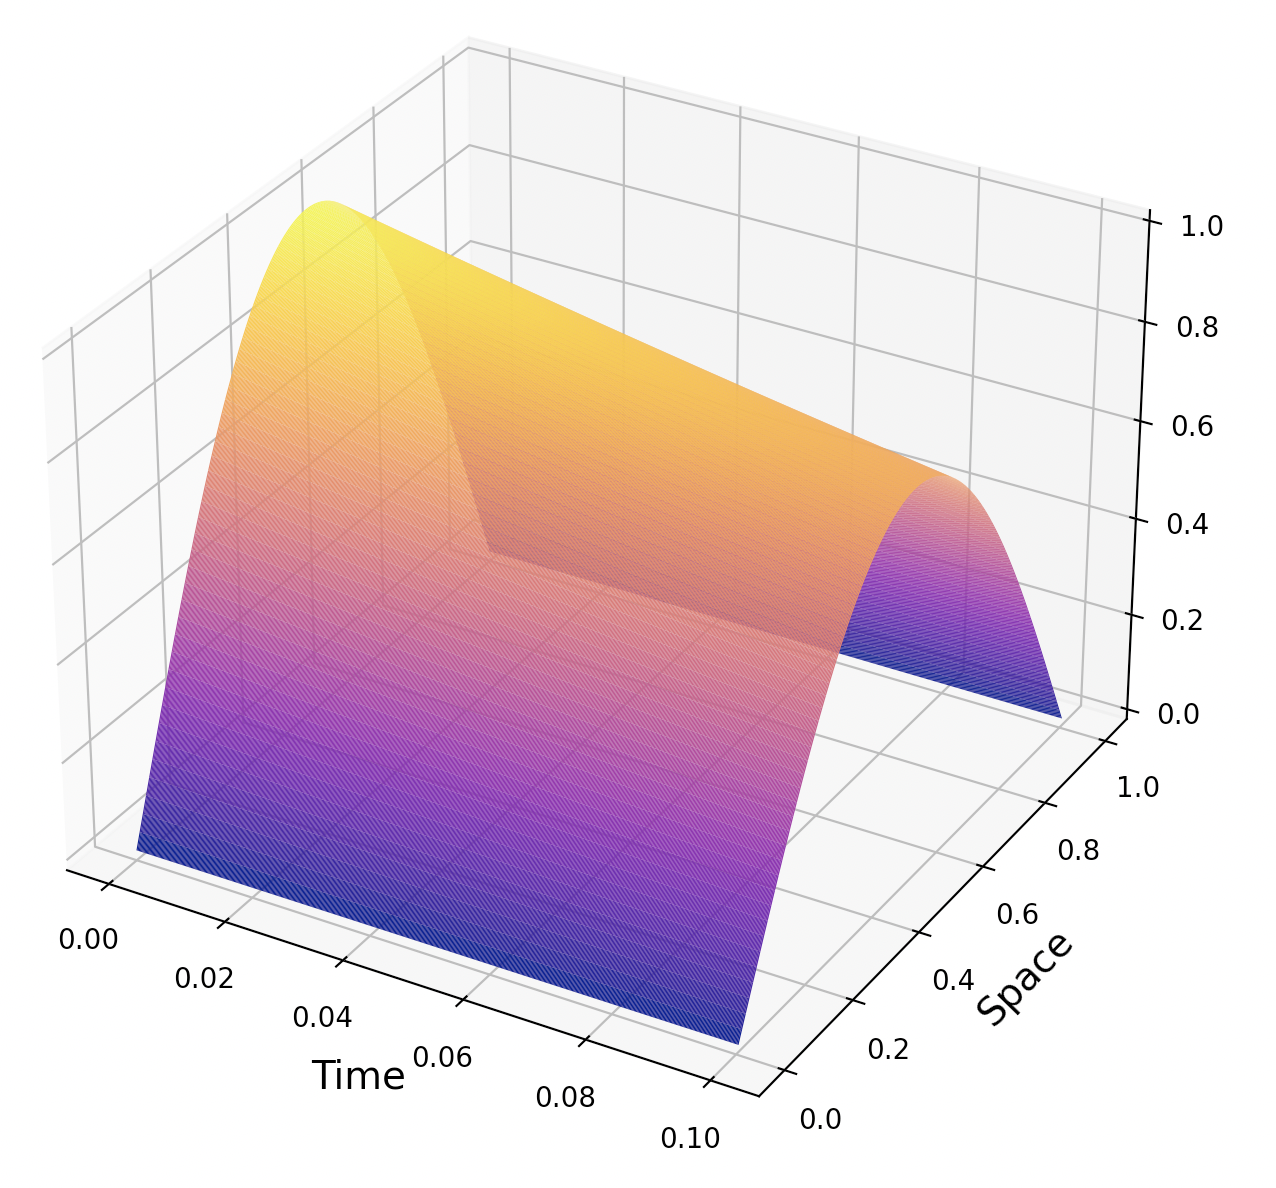
\includegraphics[scale=.2]{lambda0} \quad  $\lambda = .1$ 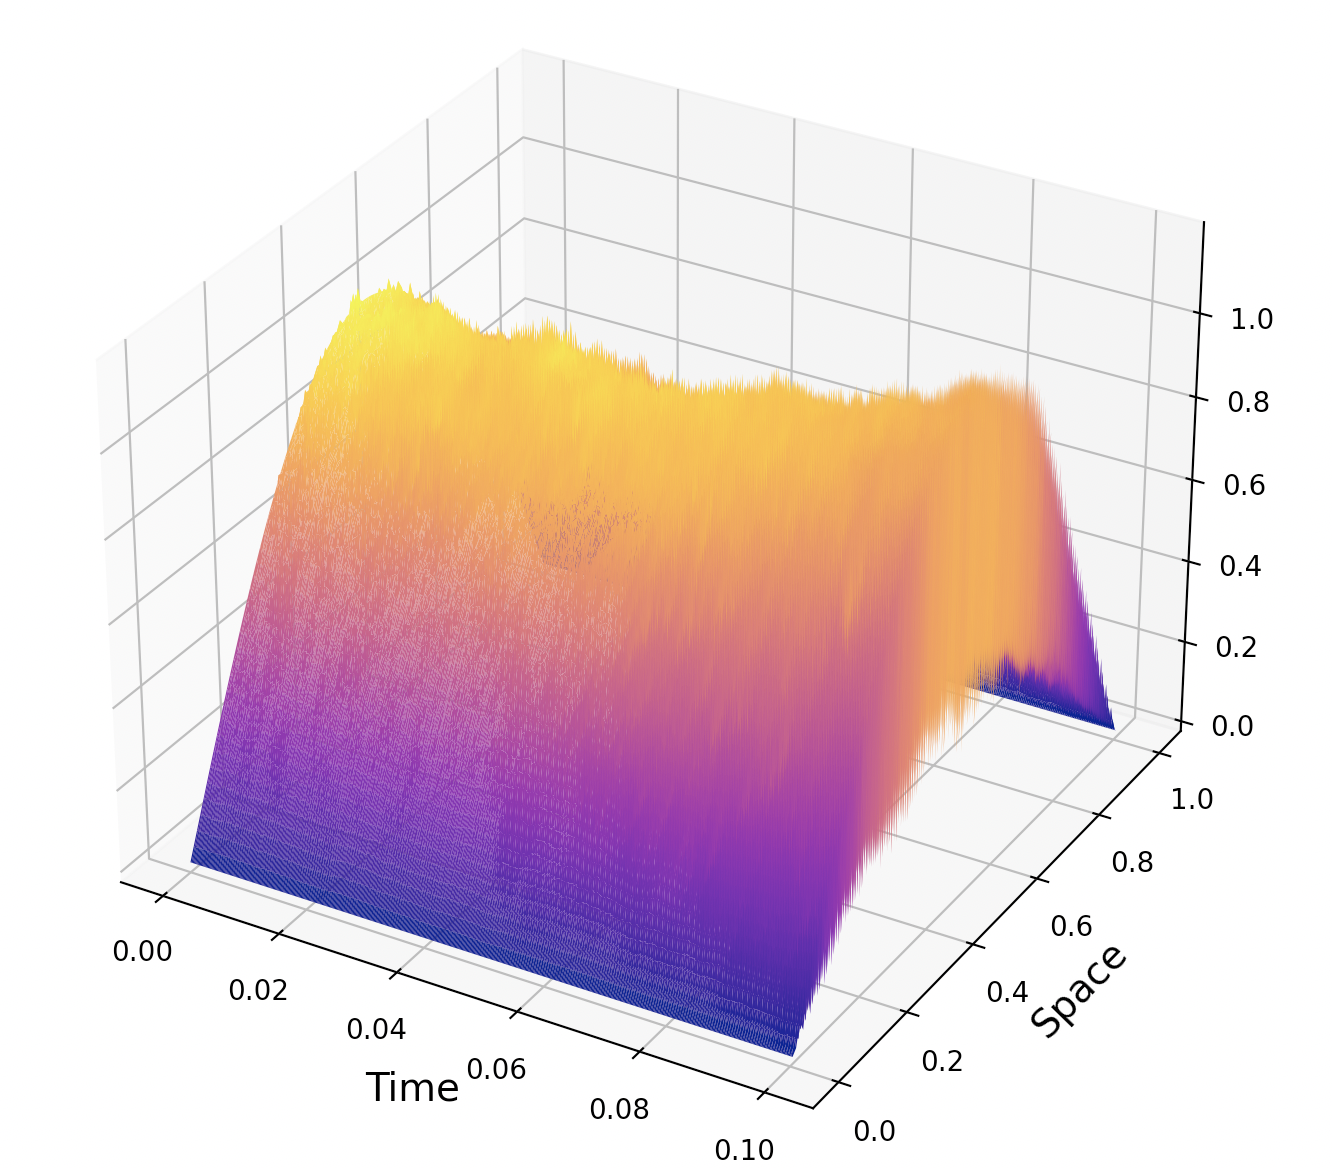
\includegraphics[scale=.2]{lambdasmall}
	
	$\lambda = 1$ 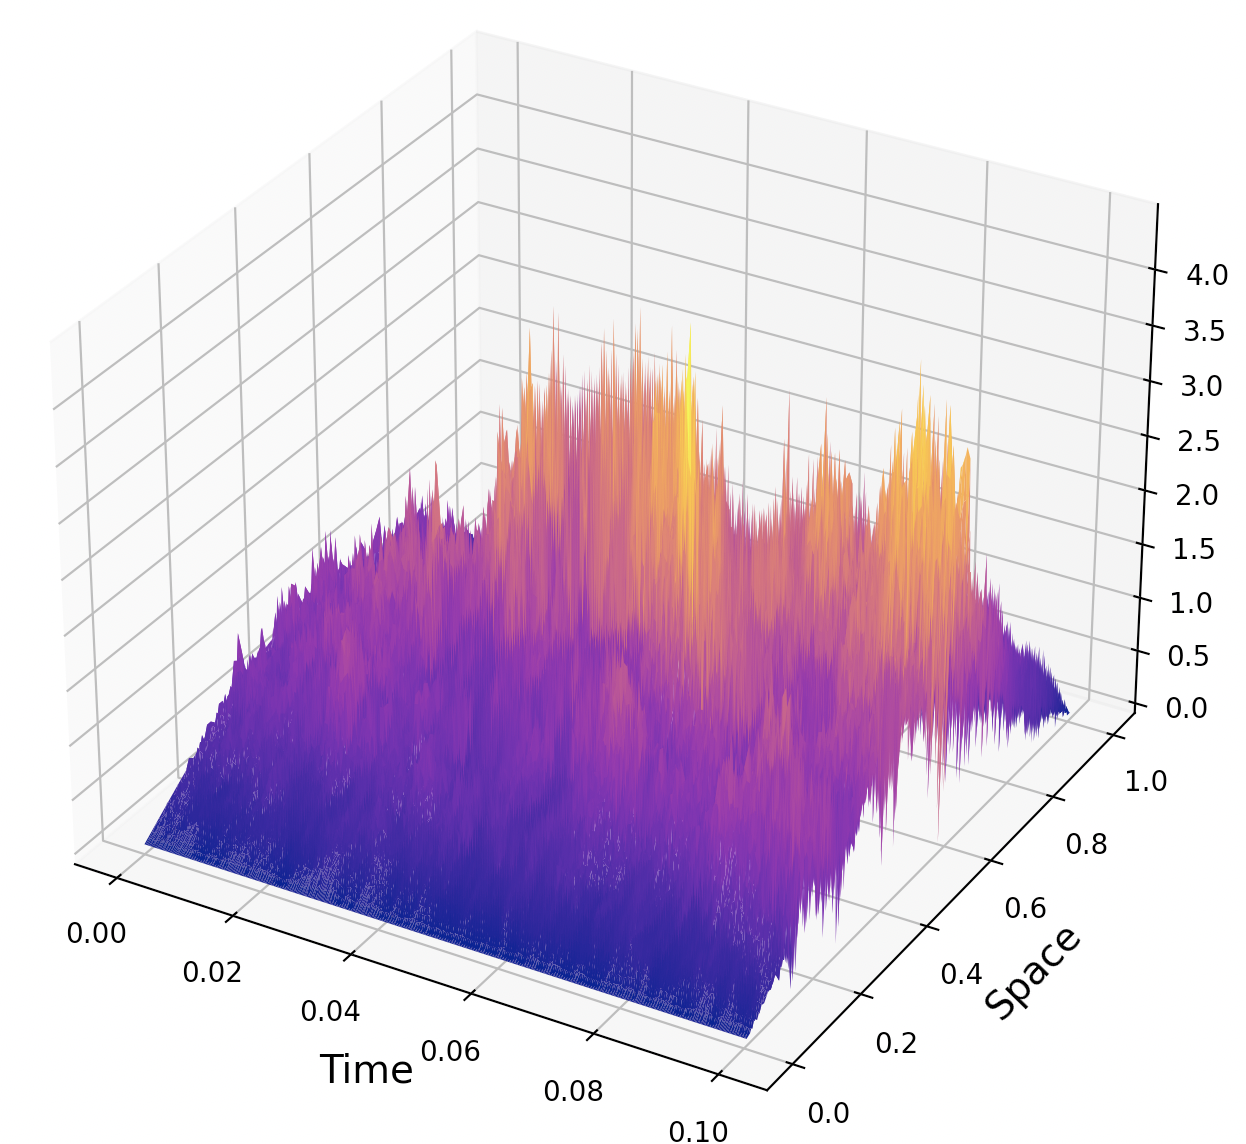
\includegraphics[scale=.2]{lambda1} \quad $\lambda = 4$ 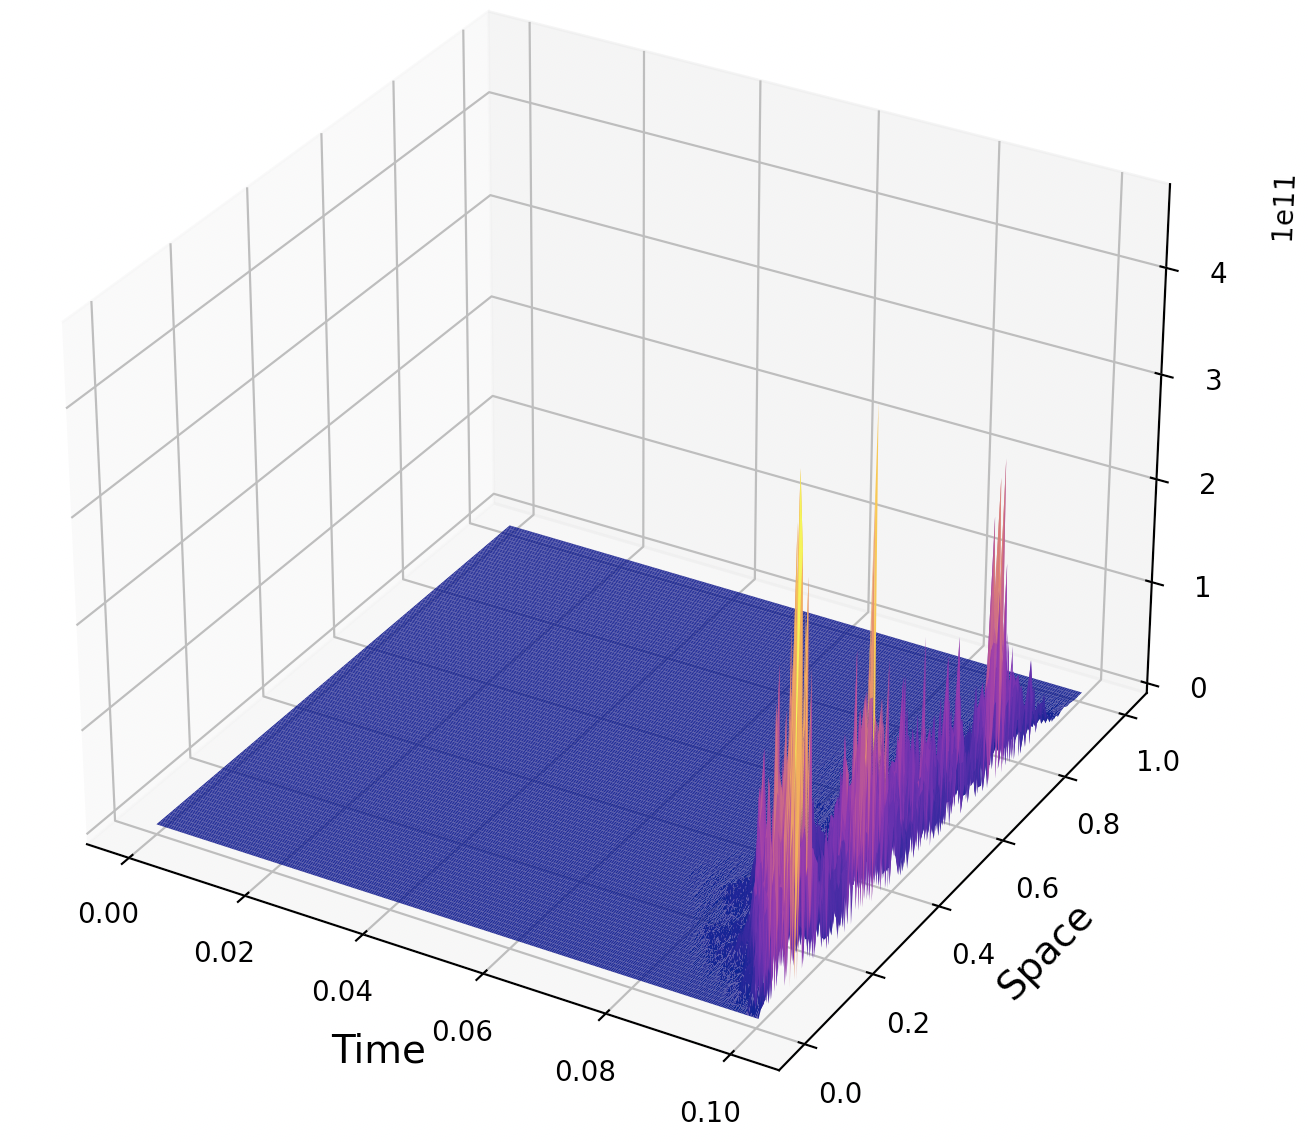
\includegraphics[scale=.2]{lambda4}
	\end{center}
\end{frame}

\begin{frame}{Bounded Moments}
	Under the assumptions for existence and uniqueness, we have the following moment bound
	\[
	\Norm{u(t,x)}_p \le C[1 + J_+(t,x)]H(t;\gamma_p)^{1/2}, \quad \gamma_p = 32pL_b^2,
	\]
	where $t\mapsto H(t,\gamma_p)$ is nondecreasing. Following a strategy laid out by Daprato and Zabczyk, we wish to prove that 
	\[
	\sup_{t \ge 0} \mathbb{E}\left( \Norm{u(t,x)}_{L^2_{\rho}(\R^d)}^2 \right) < \infty .
	\]
	Hence, a phase transition must occur. By Theorem 1.3, this forces us to require $d \ge 3$ and $\Upsilon(0) < \infty$. If we further assume that $L_b$ is small then we may also say 
	\[
	\Norm{u(t,x)}_p \le C[1 + J_+(t,x)].
	\]
	
\end{frame}

\begin{frame}[t]
	\frametitle{Invariant Measures}
Consider a measure space $(E, \mathscr{E})$ and denote $\mathcal{M}_1(E)$ to be the set of probability measure on this space.
	\begin{definition} [Invariant Measure]
		A measure $\eta(\cdot) \in \mathcal M_1(E)$ is invariant for transition functions $\{P_t(x,\Gamma)\} _{t\ge 0}$ if for any $\Gamma \in \mathscr E$ we have that $$ \eta(\Gamma) = \int_E P_t(x,\Gamma)\eta(\ud x) \quad \text{for any $t\ge 0$} $$
	\end{definition}
	
	Recall from Calculus that the average of a function $f:[a,b] \to \R$ is defined as
	$$ \text{AVG}(f) = \dfrac{1}{a-b}\int_a^b f(x) \ud x$$
	Thus,  $\eta(\Gamma)$ is the average the family of probability measures $\{P_t(x,\Gamma)\}_{x \in E}$ for any $t \ge 0$.
	
\end{frame}

\begin{frame}{Theorem: Existence of an Invariant measure}
	A processes $u(t,\cdot)(\omega)$ is bounded in probability in $L^2_{\rho}(\R^d)$ if
	\[
	\forall \epsilon >0, \; \exists R>0: \; \forall t>0, \; \mathbb{P}\left\{ \Norm{u(t,\cdot)}_{L^2_{\rho}(\R^d)} \ge R \right\} \le \epsilon.
	\] 	
	
	Tessitore and Zabczyk proved the following: \vspace{.1in}
	\begin{theorem}
		Suppose $d \ge 3$ and that there exists a $p \in [1,d/(d+2))$ such that the spatial correlation density $\gamma \in L^p(\R^d)$. Suppose that there exists two weights, $\rho$ and $\hat{\rho}$ and an element $\phi \in L^2_{\rho}(\R^d) \cap L^2_{\hat{\rho}}(\R^d)$ such that 
		\[
		\frac{\rho}{\hat{\rho}} \in L^1(\R^d) \quad \text{and} \quad u^\phi(t,\cdot) \text{is bounded in probability in} L^2_{\hat{\rho}} .
		\]
		Then there exists an invariant measure in $L^2_{\rho}(\R^d)$. 
	\end{theorem}
\end{frame}

\begin{frame}{Sketch of the Proof of Existence}
	It has been shown by DaPrato and Zabczyk that $P_t(\phi,\Gamma) := \mathscr{L}(u^\phi(t,\cdot))(\Gamma)$ defines a Markov transition function on $(L^2_{\rho}(\R^d), \mathscr{L})$ where,	
		\[
		\mathscr{L}(u^\phi(t,\cdot))(\Gamma) = \mathbb{P}\left[\omega \in \Omega : u^\phi(t,\cdot)(\omega) \in \Gamma \right], \quad \Gamma \in \mathscr{L}.
		\]
	We then prove for any $\epsilon \in (0,1)$ and $R>0$, the existence of a compact set, $\mathcal{K} \in \mathscr{L}$ such that 
		\[
				\mathscr{L}(u^\phi(t,\cdot))(\mathcal{K}) \ge (1-\epsilon)\mathbb{P}\left[\omega \in \Omega : \Norm{u^\phi(t-1,\cdot)(\omega)}_{L^2_{\rho}(\R^d)} < R \right], \quad t \ge 1.
		\]
	If we assume $u^\phi(t,\cdot)$ is bounded in probability in $L^2_{\rho}(\R^d)$ then one can argue the existence of a sequence $\{T_n\}$ such that $0<T_n \uparrow \infty$ 
		\[
				\frac{1}{T_n} \int _{t_0}^{T_n + t_0} 	\mathscr{L}(u^\phi(t,\cdot))(\Gamma) \xrightarrow[weakly]{} \eta(\Gamma) \quad \forall \Gamma \in \mathscr{L},
		\] 
	and moreover, $\eta$ is invariant in $L^2_{\rho}(\R^d)$.
		
\end{frame}


\begin{frame}{Tessitore and Zabczyk's Further Assumption}
	If $B:=\sup_{t \ge 0} \mathbb{E}\left( \Norm{u(t,x)}_{L^2_{\rho}(\R^d)}^2 \right) < \infty$ then by Chebyshev's inequality 
	\[
		\mathbb{P}[|u(t,\cdot)|_\rho \ge R] \le R^{-2}\E |u(t,\cdot)|_\rho^2 \le R^{-2}B < \epsilon, \quad \text{for any } R \ge \sqrt{B/\epsilon}.
	\]
	\begin{theorem}
		Suppose that $d \ge 3$ and that $L < L_b^{-2}$ where 
		\[
			\tilde{\Gamma} := \left|\widehat{\gamma^{1/2}}\right| * \left|\widehat{\gamma^{1/2}}\right| \quad \text{and} \quad L:= \frac{\Gamma(d/2-1)}{4\pi^{d/2}}\int_{\R^d} \tilde\Gamma(\zeta) |\zeta|^{2-d} \ud \zeta < \infty.
		\]
		Then for any admissible weight $\rho$, we have that 
			\[
			\sup_{t \ge 0} \mathbb{E}\left( \Norm{u^{\bf 1}(t,x)}_{L^2_{\rho}(\R^d)}^2 \right) < \infty.
			\]
	\end{theorem}
	\end{frame}

\begin{frame}{Moment Bound: Measure Valued Initial Conditions}
\begin{Theorem}
	Suppose that the initial measure, $\mu$, and spectral measure, $\hat{f}$:
	\begin{equation}
	\label{A:weak}
		\sup_{x\in \R^d}	\big(G(t,\cdot)*|\mu|)(x) \big) < \infty \quad \forall t>0 \quad \text{and} \quad \Upsilon(0) < \infty.
	\end{equation}
	Then if $\mu(\ud x) = \phi(x) \ud x$ with $\phi \in L^2_{\rho}(\R^d)$,
	\[
		\sup_{t \ge 0} \mathbb{E}\left( \Norm{u^\phi(t,x)}_{L^2_{\rho}(\R^d)}^2 \right) < \infty.
	\]
	Further, if $\mu$ has no density but we strengthen \eqref{A:weak} to include
		\[
		\int_0^s \ud r \: r^{-2\alpha} \int_{\R^{d}} \hat f(\ud \xi) \exp\left(-r|\xi|^2 \right) < \infty
		\]
	then for any $t_0 >0$,
		\[
			\sup_{t \ge t_0} \mathbb{E}\left( \Norm{u^\mu(t,x)}_{L^2_{\rho}(\R^d)}^2 \right) < \infty.
		\]
\end{Theorem}
\end{frame}

\begin{frame}{Invariant Measures: Measure Valued Initial Conditions}
We wish prove the existence of an invariant measure for measure valued initial conditions such as the Dirac delta measure, $\delta_0(\cdot)$. Our plan is to consider 
	\[
	\begin{cases}
	\dfrac{\partial u}{\partial t}(t,x)- \frac{1}{2}\Delta_xu(t,x) = b(x, u(t,x))\dot{W}(t,x) &
	\\ u(0,\cdot) = \mu(\cdot)  &
	\end{cases} \vspace{.1in}
	\]
and then restart our system. In other words, we will consider 
			\[
	\begin{cases}
	\dfrac{\partial v}{\partial t}(t,x)- \frac{1}{2}\Delta_xv(t,x) = b(x, v(t,x))\dot{W}(t,x) &
	\\ v(0,\cdot) = u(t_0,\cdot)  &
	\end{cases} \vspace{.1in}.
	\]
With the absence of noise, we know that $v(t,x) = u(t+t_0,x)$ and we wish to show that this property holds with the addition of noise. We also know that $\sup_{t\ge0}\Norm{u(t+t_0,\cdot)}_{L^2_{\rho}(\R^d)} < \infty$. Thus we need to figure out how extend the known proof to handle random initial conditions. 
\end{frame}










	
	
	
	\begin{frame}
		\begin{center}
			Project 2: \\
			The Interpolated Stochastic Head and Wave Equation: Sovability and Exact Moment Asymptotics
		\end{center}
	\end{frame}
	
	
	\begin{frame}[t]% {{{ SHE and SWE
		\frametitle{The Stochastic Heat and Wave Equations}
		
		\begin{equation*}
		\begin{cases}
		\left(\partial^b_t  -\Delta \right)\: u(t,x) =  u(t,x)\: \dot W(x) & \text{$x\in \R^d$, $t>0$} \\
		u(0,\cdot) = 1                                                     & b=1 \quad \text{(SHE)}    \\
		u(0,\cdot) = 1, \quad \partial_t u(0,\cdot) = 0                    & b=2 \quad \text{(SWE)}
		\end{cases}
		\end{equation*}
		
		\vfill
		\begin{itemize}
			\item $W = \{ W(\phi) : \phi \in \mathcal{D}(\R^d) \}$ is a centered and time-independent Gaussian noise
			\bigskip
			\item The choice of initial condition is such that the solution to the homogeneous equation is constant one.
			\bigskip
			\item The solution is understood in the {\it Skorohod} sense.
		\end{itemize}
		
	\end{frame}% }}}
	\begin{frame}{Known Results}% {{{ Two Known results.
		% \begin{equation*}
		% \begin{cases}
		% 	\frac{\partial^b u}{\partial t^b}(t,x) = \Delta u(t,x) +  u(t,x)\: \dot W(x) & \text{$x\in \R^d$, $t>0$}, \\
		% 	u(0,\cdot) = 1                                                               & b =1 \text{ (SHE)}         \\
		% 	u(0,\cdot) = 1, \quad \partial_t u(0,\cdot) = 0                              & b =2 \text{ (SWE)},
		% \end{cases}
		% \end{equation*}
		\begin{center}
			For the SHE, i.e., \textcolor{cyan}{$b=1$} ($a=2$, $\nu=2$)\\
			{\small [X. Chen '17]}
			\[
			\lim_{t\to \infty}t^{-\frac{4-\alpha}{2-\alpha}}\log \mathbb{E}|u(t,x)|^p =p(p-1)^{\frac{2}{2-\alpha}} (2-\alpha)\left(\frac{2\mathcal{M}}{4-\alpha}\right)^{\frac{4-\alpha}{2-\alpha}}
			\]
		\end{center}
		\vspace{.3in}
		\begin{center}
			For the SWE, i.e., \textcolor{cyan}{$b=2$} ($a=2$, $\nu=2$)\\
			{\small [Balan, L. Chen, and X. Chen '21]}
			\[
			\lim_{t \to \infty} t^{-\frac{4-\alpha}{3-\alpha}} \log \mathbb{E}|u(t,x)|^p =p(p-1)^{\frac{1}{3-\alpha}} \left(\frac{1}{2}\right)^{\frac{\alpha}{2(3-\alpha)}} \frac{3- \alpha}{2} \left( \frac{2 \mathcal{M}^{1/2}}{4-\alpha} \right)^{\frac{4-\alpha}{3-\alpha}}
			\]
		\end{center}
		
	\end{frame}% }}}
	
	\begin{frame}[t]%{{{ ISHWE
		\frametitle{The Interpolated Stochastic Heat and Wave Equation}
		\begin{equation}
		\tag{\footnotesize ISHWE}
		\begin{cases}
		\left(\partial^b_t + \frac{\nu}{2}(-\Delta)^{a/2}\right) u(t,x) = I^r_t \left[\sqrt{\theta}\: u(t,x)\: \dot W(x) \right] & \text{$x\in \R^d$, $t>0$} \\
		u(0,\cdot) = 1                                                                                                           & b \in (0,1]               \\
		u(0,\cdot) = 1, \quad \partial_t u(0,\cdot) = 0                                                                          & b \in (1,2)
		\end{cases}
		\end{equation}
		
		\vfill
		\begin{itemize}
			\item $\partial^b_t$ is the {\it Caputo} fractional derivative
			\bigskip
			\item $(-\Delta)^{a/2}$ is the fractional Laplacian of order $a \in (0,2]$
			\bigskip
			\item $I^r_t$ is the Riemann-Liouville fractional integral of order $r \ge 0$
		\end{itemize}
		
	\end{frame}% }}}
	
	
	
	\begin{frame}[t]% {{{ Noise
		
		\frametitle{The Noise, $\dot{W}$.}
		The time independent noise informally satisfies
		\[
		\mathbb{E}(\dot{W}(x)\dot{W}(y)) = \gamma(x-y).
		\]
		The spatial correlation and spectral density, $\gamma$ and $\varphi$, for the noise $\dot{W}$ can be assumed to be any of the following:
		\bigskip
		\begin{align*}
		\gamma(x) & = |x|^{-\alpha}, \;                     & \varphi(\xi) & =C_1 |\xi|^{d-\alpha}                     &  & \alpha \in (0,d) \\[1em]
		\gamma(x) & = \prod_{i=1}^d |x_{i}|^{-\alpha_i}, \; & \varphi(\xi) & = C_2\prod_{i=1}^d |\xi_{i}|^{1-\alpha_i} &  & \alpha_i \in (0,1),\: \alpha = \sum_i\alpha_i
		\end{align*}
		% \[ \gamma(x) = \prod_{i=1}^k |x_{(i)}|^{-\alpha_i}, \; \varphi(\xi) = C_3\prod_{i=1}^k |\xi_{(i)}|^{d_i-\alpha_i}\text{ where } \alpha_i \in (0,d_i)\]
		% In the second two cases we define $\alpha = \sum_i\alpha_i$.
	\end{frame}% }}}
	
	
	\begin{frame}[t]
		\frametitle{Mild Solution}
		\begin{definition}
			For $T > 0$, a random field $u=\{u(t,x): t \in (0,T), x \in \R^d \} $ is called a \textit{mild solution} if $G(t-s,x-\cdot)u(s,\cdot)1_{\{s<t\}}$ is Skorohod integrable and the following holds almost surely:
		\end{definition}
		\[
		u(t,x) = 1 + \sqrt{\theta} \int_0^t \left(\int_{\R^d} G(t-s,x-y)u(s,y)W(\delta y)\right) \ud s
		\]
		where $G$ is defined through the \textit{Fox-H function}.
		\\ $\;$ \\
		An important characteristic of $G$ is that
		\[
		\mathcal{F}\mathcal{L}G(s,\xi) = \frac{s^{-r}}{s^{b}+\frac{\nu}{2}|\xi|^a}
		\]
	\end{frame}
	
	\begin{frame}[t]
		\frametitle{Nonnegativity assumption on $G$}
		Under any of the following cases, $G$ is nonnegative {\small [Chen, Hu, Nualart '19]}:
		\begin{itemize}
			\item $d \ge 1$, $b\in(0,1]$, $a\in(0,2]$, $r\ge0$;
			% \item $d \ge 1$, $b=1$, $a\in (0,2]$, $r=0$ or $r>1$;
			\item $1\le d \le 3$, $1<b<a\le 2$, $r>0$;
			\item $1 \le d \le 3$, $1 < b=a < 2$, $r > \dfrac{d+3}{2}-b$.
		\end{itemize}
		\begin{figure}[htpb]
			\centering
			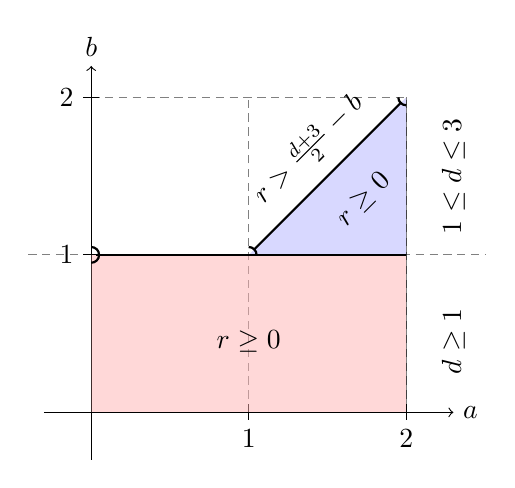
\begin{tikzpicture}[scale=2]
			\draw [->] (-0.3,0) -- (2.3,0) node [right] {$a$};
			\draw [->] (0,-0.3) -- (0,2.2) node [above] {$b$};
			\draw [densely dashed,gray] (1,0) -- (1,2) (2,0) -- (2,2) (-0.4,1) -- (2.5,1) (0,2) -- (2,2);
			\draw (1,0.05) -- (1,-0.05) node [below] {$1$};
			\draw (2,0.05) -- (2,-0.05) node [below] {$2$};
			\draw (0.05,1) -- (-0.05,1) node [left] {$1$};
			\draw (0.05,2) -- (-0.05,2) node [left] {$2$};
			\filldraw [fill=red!30, opacity=0.5] (0,0) rectangle (2,1);
			\filldraw [fill=blue!30, opacity=0.5] (1,1) -- (2,1) -- (2,2);
			\draw [thick] (1.03,1.03) -- (1.97,1.97);
			\draw [thick] ([shift=(0:0.05)]1,1) arc (0:90:0.05);
			\draw [thick] ([shift=(180:0.05)]2,2) arc (180:270:0.05);
			\node at (2.3,1.5) [rotate=90, anchor=center] {$1\le d\le 3$};
			\node at (2.3,0.45)[rotate=90, anchor=center] {$d\ge 1$};
			\draw [thick] (0.03,1) -- (2,1);
			\draw [thick] ([shift=(-90:0.05)]0,1) arc (-90:90:0.05);
			\node at (1.73,1.35) [rotate=45, anchor=center] {$r\ge 0$};
			\node at (1,0.45) {$r\ge 0$};
			% \node at (1,0.9) {$r=0$ or $r>1$};
			\node at (1.5,1.55) [rotate=45,anchor=south] {$r>\frac{d+3}{2}-b$};
			\end{tikzpicture}
		\end{figure}
	\end{frame}
	
	\begin{frame}
		\frametitle{Global Solution\\
			\small $\left(\partial^b_t + \frac{\nu}{2}(-\Delta)^{a/2}\right)\: u(t,x) = I^r_t \left[\sqrt{\theta}\: u(t,x)\: \dot W(x) \right]$}
		\begin{definition}
			$u(t,x)$ is a \textit{global solution} to the {\small (ISHWE)} if $\Norm{u(t,x)}_p < \infty$ for any $t>0$ and $x \in \R^d$.
		\end{definition}
		$\;$ \\
		\begin{theorem}[{\small Chen-E. '21+}]
			A global solution exists provided $G$ is nonnegative and
			\[
			0 < \alpha < \min\left( \frac{a}{b}[2(b+r) -1], 2a, d \right)
			\]
		\end{theorem}
	\end{frame}
	
	\begin{frame}
		\frametitle{Local Solution}
		\begin{definition}
			$u(t,x)$ is a \textit{local solution} to the {\small (ISHWE)} if there exists $0 < T_a \le T_b < \infty$ such that $\Norm{u(t,x)}_2 < \infty$ when $0<t<T_a$ and $\Norm{u(t,x)}_2 $ D.N.E. (does not exist) for $t> T_b$.
		\end{definition}
		$\;$ \\
		\begin{theorem}[{\small Chen-E. '21+}]
			A local solution exists provided $G$ is nonnegative and
			if
			\[
			r\in \left[0,1/2\right] \qquad \text{and} \qquad
			0<\alpha = \frac{a}{b}[2(b+r)-1] \le d.
			\]
			In this case, a unique $L^p(\Omega)$ solution exists for $t \in (0,T_p)$ where
			\[
			T_p := \dfrac{\nu^{\alpha/a}}{2 \theta (p-1) \mathcal{M}_a^{(2a-\alpha)/a}}
			\]
			and the solution does not exist for $t > T_2$.
		\end{theorem}
	\end{frame}
	
	
	
	\begin{frame}[t]
		\frametitle{Example: Solvability for the SWE ($a=b=2$)}
		A local solution only exists when $\alpha = 3+2r \le d \le 3$.
		\begin{figure}[htb]% {{{ F:SWE
			\centering
			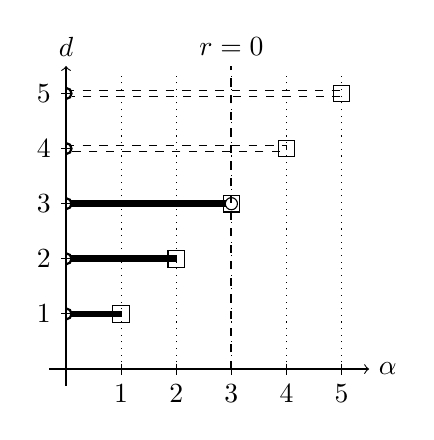
\begin{tikzpicture}[scale=0.7]
			\draw [thick,dashed] (3,0) -- (3,5.5) node [above] {$r=0$};
			\draw [->] (-0.3,0) -- (5.5,0) node [right] {$\alpha$};
			\draw [->] (0,-0.3) -- (0,5.5) node [above] {$d$};
			\foreach \x in {1,...,5}{
				\draw (\x,0.1)--++(0,-0.2) node [below] {$\x$};
				\draw (0.1,\x)--++(-0.2,0) node [left] {$\x$};
				\draw (\x,\x) + (-0.15,-0.15) rectangle +(0.15,0.15);
				\draw [thick] ([shift=(-90:0.1)]0,\x) arc (-90:90:0.1);
				\draw [thin, dotted] (\x,0) -- (\x, 5.4);
			}
			\filldraw (0, 1) + (0.1, -0.05) rectangle +(1,0.05);%\filldraw (1,1) circle (0.05);
			\filldraw (0, 2) + (0.1, -0.05) rectangle +(2,0.05);%\filldraw (2,2) circle (0.05);
			\filldraw (0, 3) + (0.1, -0.05) rectangle +(2.9,0.05);%\filldraw (3,3) circle (0.05);
			% \filldraw (0, 4) + (0.1, -0.05) rectangle +(2.9,0.05);
			% \filldraw (0, 5) + (0.1, -0.05) rectangle +(2.9,0.05);
			% \draw (2,2) circle (0.11);
			\draw (3,3) circle (0.11);
			% \draw (3,4) circle (0.11);
			% \draw (3,5) circle (0.11);
			% \draw (2, 3) + (0.1, -0.05) rectangle +(1,0.05);
			% \draw (2, 4) + (0.1, -0.05) rectangle +(2,0.05);
			\draw[dashed] (0, 5) + (0.1, -0.05) rectangle +(5,0.05);
			\draw[dashed] (0, 4) + (0.1, -0.05) rectangle +(4,0.05);
			\end{tikzpicture}
			\hspace{2em}
			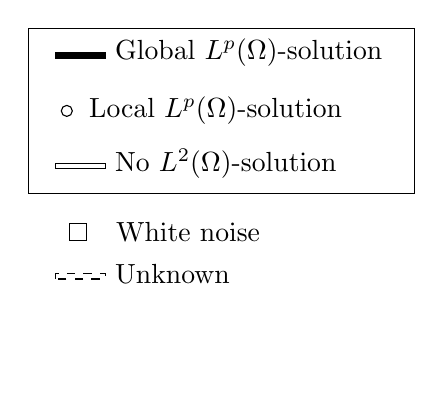
\begin{tikzpicture}[scale=0.7]
			\def\x{3.2}
			% \draw (-0.4,-1.5+\x) rectangle +(6,3);
			% \draw (0.5,0+\x) circle (0.1); \node at (3,0+\x) {Local $L^p(\Omega)$-solution};
			% \draw (0, -1+\x) + (0.1, -0.05) rectangle +(1,0.05) node [right] {No $L^2(\Omega)$-solution};
			% \draw (0.5, 1) + (-0.15,-0.15) rectangle +(0.15,0.15); \node at (2.5,1) {White noise};
			\draw[dashed] (0, -3+\x) + (0.1, -0.05) rectangle +(1,0.05) node [right] {Unknown};
			\draw (-0.4,-1.5+\x) rectangle +(7,3);
			\filldraw (0, 1+\x) + (0.1, -0.05) rectangle +(1,0.05) node [right] {Global $L^p(\Omega)$-solution};
			\draw (0.3,0+\x) circle (0.1); \node at (3,0+\x) {Local $L^p(\Omega)$-solution};
			\draw (0, -1+\x) + (0.1, -0.05) rectangle +(1,0.05) node [right] {No $L^2(\Omega)$-solution};
			\draw (0.5, 1) + (-0.15,-0.15) rectangle +(0.15,0.15); \node at (2.5,1) {White noise};
			\draw[white] (0,-1.5) circle (0.01);
			\end{tikzpicture}
		\end{figure}% }}}
		By replacing $\nu=2$ in the following, we recover (1.12) {\small [Balan, L. Chen \& X. Chen '21]}
		\[
		T_p=	\frac{\nu^{3 / 2}}{2\theta (p-1) \sqrt{\mathcal{M}_{2,3}(\delta_0)}},  \quad p\ge 2
		\]
	\end{frame}
	
	
	\begin{frame}[t]
		\frametitle{Example: Solvability for the SHE ($a=2$ and  $b=1$)}
		By setting $a=2$, $b=1$ and $r=0$, we obtain the following condition for existence of a local solution: $\alpha = 2 \le d.$
		\begin{columns}
			\begin{column}{0.5\textwidth}
				\begin{figure}[htpb]% {{{ F:SHE
					\centering
					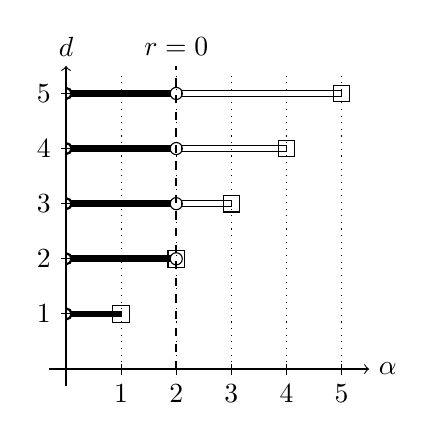
\begin{tikzpicture}[scale=0.7]
					\draw [thick,dashed] (2,0) -- (2,5.5) node [above] {$r=0$};
					\draw [->] (-0.3,0) -- (5.5,0) node [right] {$\alpha$};
					\draw [->] (0,-0.3) -- (0,5.5) node [above] {$d$};
					\foreach \x in {1,...,5}{
						\draw (\x,0.1)--++(0,-0.2) node [below] {$\x$};
						\draw (0.1,\x)--++(-0.2,0) node [left] {$\x$};
						\draw (\x,\x) + (-0.15,-0.15) rectangle +(0.15,0.15);
						\draw [thick] ([shift=(-90:0.1)]0,\x) arc (-90:90:0.1);
						\draw [thin, dotted] (\x,0) -- (\x, 5.4);
					}
					\filldraw (0, 1) + (0.1, -0.05) rectangle +(1,0.05);%\filldraw (1,1) circle (0.05);
					\filldraw (0, 2) + (0.1, -0.05) rectangle +(1.9,0.05);
					\filldraw (0, 3) + (0.1, -0.05) rectangle +(1.9,0.05);
					\filldraw (0, 4) + (0.1, -0.05) rectangle +(1.9,0.05);
					\filldraw (0, 5) + (0.1, -0.05) rectangle +(1.9,0.05);
					\draw (2,2) circle (0.11);
					\draw (2,3) circle (0.11);
					\draw (2,4) circle (0.11);
					\draw (2,5) circle (0.11);
					\draw (2, 3) + (0.1, -0.05) rectangle +(1,0.05);
					\draw (2, 4) + (0.1, -0.05) rectangle +(2,0.05);
					\draw (2, 5) + (0.1, -0.05) rectangle +(3,0.05);
					\end{tikzpicture}
				\end{figure}
			\end{column}
			\begin{column}{0.5\textwidth}
				\begin{itemize}
					\item 	When $\alpha=d=2$, the critical time becomes $T_p = \dfrac{\nu}{2\theta (p-1) \mathcal{M}_{2,2}(\delta_0)}$.
					\item Theorem 4.1 {\small [Y. Hu, '01]} proves that an $L^2(\Omega)$ solution exists for $t<2$ but not for $t>2 \pi$.
					\item $T_2$ being precise implies $2 \le T_2 = \frac{1}{2\mathcal{M}_{2,2}(\delta_0)} \le 2\pi$
				\end{itemize}
			\end{column}
		\end{columns}
		
	\end{frame}
	
	\begin{frame}[t]
		\frametitle{Wiener Chaos Expansion}
		
		Through a standard procedure, we may define
		\[
		f_n(x_1, \cdots , x_n; x, t) = \int_0^t\int_0^{t_n}\cdots \int_0^{t_2} \prod_{k=1}^n G(t_{k+1}-t_k,x_{k+1}-x_k) \ud t_1 \cdots \ud t_n
		\]
		where $t=t_{n+1}$ and $x=x_{n+1}$, and say that
		\vspace{1em}
		\begin{enumerate}
			\setlength\itemsep{.8em}
			\item $u(t,x) = 1 + \sum_{k=1}^\infty \theta^{k/2} I_k(f_k(\cdot,x,t)), \quad (t,x)\in (0,T)\times \R^d$
			
			\item $\mathbb{E}(u(t,x)^2) = \sum_{k=0}^\infty \theta^{k} \Norm{f_k(\cdot,x,t)}^2_{\mathcal{H}^{\otimes n}}, \quad (t,x)\in (0,T)\times \R^d$.
		\end{enumerate}
		\vspace{1em}
		Through a change of variable, one can easily show that
		\vspace{1em}
		\begin{enumerate}
			\item $\mathcal{F}G(t,\cdot)(c\xi) = c^{-\frac{a}{b}(b+r -1)}\mathcal{F}G\left(c^{\frac{a}{b}}t,\cdot\right)( \xi)$
			\item $\Norm{\widetilde{f_n}(\cdot,0,t)}_{\mathcal{H}^{\otimes n}}^2 = t^{[2(b + r ) -b \alpha / a]n} \Norm{\widetilde{f_n}(\cdot,0,1)}_{\mathcal{H}^{\otimes n}}^2$
		\end{enumerate}
	\end{frame}
	
		\begin{frame}[t]
		\frametitle{How to Find the Critical $\alpha$}
		For simplicity we consider the SWE ($a=b=2$ and $r=0$).
		\begin{align*}
		\Norm{u(t,x)}_2^2 &= \sum_{n \ge 0} \theta^n n! \: \overbrace{t^{[4 - \alpha ]n}  \Norm{ \widetilde{f_n}(\cdot,0,1) }_{ \mathcal{H}^{\otimes n} }^2}^{\Norm{ \widetilde{f_n}(\cdot,0,t) }_{ \mathcal{H}^{\otimes n} }^2}
		\\&\le \sum_{n \ge 0} \frac{(\theta t^{4-\alpha}c_12^{4-\alpha} C_\mu)^n }{(n!)^{3-\alpha}}  , \quad C_\mu = \int_{\R^d} \left(\frac{1}{1+|\xi|^2}\right)^2 \mu(\ud \xi) < \infty
		\end{align*}
		When $\alpha = 3$, then the above reduces down to, we lose the $n!$ term in the denominator. 
	\end{frame}
	
		\begin{frame}[t]
		\frametitle{How to Find the Blowup Time (SWE)}
		Recall from above that the critical case corresonds to $\alpha = 3 = d$.
		\begin{align*}
		\Norm{u(t,x)}_2^2 &= \sum_{n \ge 0} \theta^n n! \Norm{\tilde{f}(\cdot,0,t)}_{H^{\otimes n}}^2
		\\&= \sum_{n \ge 0} (\theta t)^n n! \Norm{\tilde{f}(\cdot,0,1)}_{H^{\otimes n}}^2
		\\& =: \sum_{n \ge 0} (\theta t)^n R_n, \quad R_n = n! \Norm{\tilde{f}(\cdot,0,1)}_{H^{\otimes n}}^2.
		\end{align*}
		The lemma below says that $\frac{1}{n}\log{R_n} \to \log(2 \rho)$. Now the Cauchy-Hadamard theorem can be directly applied to see that the radius of convergence is precisely $(2\theta \rho)^{-1} = T_2$.
		
	\end{frame}
	
	\begin{frame}
		Recall the scaling property
		\[
		\Norm{\tilde{f}_n(\cdot,0,t)}_{\mathcal{H}^{\otimes n}}^2 = t^{(4-\alpha)n}\Norm{\tilde{f}_n(\cdot,0,1)}_{\mathcal{H}^{\otimes n}}^2.
		\]
		Using this scaling property we see that
		\[
		\int_0^\infty e^{-t}\Norm{\tilde{f}_n(\cdot,0,t)}_{\mathcal{H}^{\otimes n}}^2  \ud t = \Gamma((4-\alpha)n+1)\Norm{\tilde{f}_n(\cdot,0,1)}_{\mathcal{H}^{\otimes n}}^2.
		\]
		
		\begin{lemma}[{\small R.  Balan, L. Chen \& X. Chen '21}]
			
			\begin{align*}
			\lim_{n \to \infty}\frac{1}{n} \log & \left(\Gamma((4-\alpha)n+1)\Norm{\tilde{f}_n(\cdot,0;1)}_{\mathcal{H}^{\otimes n}}^2\right) = \log\left[ 2^{4-\alpha}\rho \right]
			\\ \\ \lim_{n \to \infty}\frac{1}{n} \log & \left((n!)^{4-\alpha}\Norm{\tilde{f}_n(\cdot,0;1)}_{\mathcal{H}^{\otimes n}}^2\right) = \log\left[ \left(\frac{2}{4-\alpha}\right)^{4-\alpha}\rho \right]
			\end{align*}
		\end{lemma}
	\end{frame}
	
		
	\begin{frame}[t]
		\frametitle{$\rho$}
		We define
		\begin{align*}
		\rho_{\nu,a}(\gamma) &= \sup_{\Norm{f}_{L^2(\R^d)} =1} \int_{\R^d} \left[ \int_{\R^d} \frac{f(x+y)f(y)}{\sqrt{1+\frac{\nu}{2}|x+y|^a } \sqrt{1+\frac{\nu}{2}|y|^a} } \ud y \right]^2 \mu(\ud x)
		\end{align*}
		
		
		
		
		\begin{theorem}[{\small X. Chen '07}]
			\begin{align*}
			\lim_{n \to \infty} \frac{1}{n} \log & \left[ \frac{1}{(n!)^2} \int_{(\R^d)^n} \left( \sum_{\sigma \in \Sigma_n} \prod_{k=1}^n \frac{1}{1+ \frac{\nu}{2}|\sum_{j=k}^n \xi_{\sigma(j)}|^a}\right)^2 \mu (\ud \vec{\xi})\right]
			\\& = \log\left( \rho_{\nu, a}\left(\gamma\right) \right).
			\end{align*}
			where $\gamma$ is the spatial correlation function.
		\end{theorem}
		
	\end{frame}
	
	\begin{frame}[t]
		\frametitle{Connection of the SPDE with $\rho$}
		Recall from above that
		\[
		\mathcal{F}\mathcal{L}G(1,\xi) = \frac{1}{1+\frac{\nu}{2}|\xi|^a}.
		\]
		By using this relation, it can be shown that
		\[
		\mathcal{F}\mathcal{L}(\tilde{f}_n)(1,\xi) = \frac{1}{n!} \sum_{\sigma \in \Sigma_n} \prod_{k=1}^n \frac{1}{1+ \frac{\nu}{2}|\sum_{j=k}^n \xi_{\sigma(j)}|^a}.
		\]
		Applying this to the limit representation of $\rho$ above yields that
		\begin{align*}
		\lim_{n \to \infty} \frac{1}{n} \log  \left[ \int_{(\R^d)^n} \left| \mathcal{F}\mathcal{L}(\tilde{f}_n)(1,\xi)\right|^2 \mu (\ud \vec{\xi})\right]  = \log\left( \rho_{\nu, a}\left(\gamma\right) \right).
		\end{align*}
	\end{frame}
	
	\begin{frame}[t]% {{{ M
		\frametitle{$\mathcal{M}$}
		We define
		\begin{align*}
		\mathcal{M}_{a,d}(\gamma,\theta) & := \sup_{g \in \mathcal{F}_a} \left\{ \left( \iint_{\R^{2d}} g^2(x)g^2(y) \gamma(x+y)\ud x\ud y \right)^{1/2} - \frac{\theta}{2}\: \mathcal{E}_a(g,g) \right\} \\
		& = \sup_{g \in \mathcal{F}_a} \left\{ \left\langle g^2 * g^2, \gamma \right\rangle_{L^2(\R^d)}^{1/2} - \frac{\theta}{2}\: \mathcal{E}_a(g,g) \right\},
		\end{align*}
		where
		\begin{gather*}
		\mathcal{E}_a(g,g) := (2\pi)^{-d} \int_{\R^d} |\xi|^a |\mathcal{F}g(\xi)|^2 \ud \xi \quad \text{and} \\
		\mathcal{F}_a      := \left\{f\in L^2(\R^d): \: \Norm{f}_{L^2(\R^d)}=1,\: \mathcal{E}_a(f,f)<\infty \right\}.
		\end{gather*}
		
			\begin{theorem}[{\small Bass, X. Chen and Rosen '09}]
			\[
			\rho_{\nu,a}(\gamma) = \nu^{-\alpha/a} \mathcal{M}_a^{2-(\alpha / a)}(\gamma)<\infty
			\]
		\end{theorem}
	\end{frame}% }}}f
	
	\begin{frame}[t]% {{{ Moment asymptotics
		\frametitle{The Moment Asymptotic}
		\begin{theorem}[{\small Chen-E. '21+}]
			Suppose a global solution to the SPDE in question exists and $\dot{W}$ is given through the generalized Riesz kernel defined above. Then,
			\begin{align*}
			\lim_{t_p \to \infty} & t_p^{-\beta} \log \Norm{u(t,x)}_p                                          \\
			& =  \left(\frac{1}{2}\right)\left(\frac{2a}{2a(b+r)- b\alpha} \right)^\beta \\
			& \quad \quad \quad  \times \left(\theta\nu^{-\alpha/a} \mathcal{M}_a^{\frac{2a-\alpha}{a}}\right)^{\frac{a}{2a(b+r)-b\alpha-a}}\left(2(b+r)-\frac{b\alpha}{a}-1\right),
			\end{align*}
			where
			\begin{align*}
			% \label{E:beta-tp}
			\beta := \dfrac{2(b+r)-\dfrac{b\alpha}{a}}{ 2(b+r)-\dfrac{b\alpha}{a} -1 } \qquad \text{and} \qquad
			t_p   := (p-1)^{1-1/\beta} \: t.
			\end{align*}
		\end{theorem}
	\end{frame}% }}}
	
	\begin{frame}[t]% {{{ Exponential growth of moments in time
		% \frametitle{Exponential Growth of the Moments in Time}
		\frametitle{Exact Moment Lyapunov Exponent \\
			\small (Recall $\beta := \frac{2(b+r)-\frac{b\alpha}{a}}{ 2(b+r)-\frac{b\alpha}{a} -1}$)}
		\begin{corollary}[{\small Chen-E. '21+}]
			For $p \ge 2$ fixed, we have that
			\begin{align*}
			\lim_{t \to \infty} & t^{-\beta} \log \E\left(|u(t,x)|^p\right)                                                                                 \\
			& =  p(p-1)^{\frac{1}{2(b+r)-\frac{b\alpha}{a} -1}} \left(\frac{1}{2}\right)\left(\frac{2a}{2a(b+r)- b\alpha} \right)^\beta \\
			& \quad \quad \times \left(\theta\nu^{-\alpha/a} \mathcal{M}_a^{\frac{2a-\alpha}{a}}\right)^{\frac{a}{2a(b+r)-b\alpha-a}}\left(2(b+r)-\frac{b\alpha}{a}-1\right).
			\end{align*}
		\end{corollary}
		\vfill
		
		From this we can deduce that $t \mapsto \mathbb{E}(|u(t,x)|^p)$ will grow like $\exp\left({K_1 t^\beta }\right)$, in other words, the moments will grow exponentially in time,
		and we obtain the exact expression for the constant $K_1$.
	\end{frame}% }}}
	
	\begin{frame}[t]% {{{ Exact Large Moment Asymptotics
		% \frametitle{Exponential Growth of the moments for Fixed Time}
		\frametitle{Exact Large Moment Asymptotics \\
			\small (Recall $\beta := \frac{2(b+r)-\frac{b\alpha}{a}}{ 2(b+r)-\frac{b\alpha}{a} -1}$)}
		\begin{corollary}[{\small Chen-E. '21+}] For $t>0$ fixed , we have that
			\begin{align*}
			\lim_{p \to \infty} & p^{-\beta} \log \E\left(|u(t,x)|^p\right)                                          \\
			& =  t^\beta \left(\frac{1}{2}\right)\left(\frac{2a}{2a(b+r)- b\alpha} \right)^\beta \\
			& \quad \quad \times \left(\theta\nu^{-\alpha/a} \mathcal{M}_a^{\frac{2a-\alpha}{a}}\right)^{\frac{a}{2a(b+r)-b\alpha-a}}\left(2(b+r)-\frac{b\alpha}{a}-1\right).
			\end{align*}
		\end{corollary}
		\vfill
		
		From this we can deduce that $p \mapsto \mathbb{E}(|u(t,x)|^p)$ will grow like $\exp\left({K_2 p^\beta }\right)$, in other words, the moments will grow exponentially in $p$ as well.
		
	\end{frame}% }}}
	
	\begin{frame}
		\frametitle{References}
		\small
		
		\begin{thebibliography}{999}
			\bibitem{BCC21} % {{{ 1.
			Balan, R. M., Chen, L., and Chen, X. (2021).
			\newblock Exact asymptotics of the stochastic wave equation with time-independent noise.
			\newblock {\em  Ann. Inst. Henri Poincar\'e Probab. Stat. }, to appear.
			
			\bibitem{BCR09}% {{{ 2.
			Bass, R., Chen, X., and Rosen, M. (2009).
			\newblock Large deviations for Riesz potentials of additive processes.
			\newblock {\em  Ann. Inst. Henri Poincar\'e Probab. Stat. } \textbf{45}, 626--666.
			% }}}
			
			\bibitem{BCC21} % {{{ 1.
			Chen, L. and Eisenberg, N. (2021+).
			\newblock Interpolating the Stochastic Heat and Wave Equations\\ with Time-independent Noise:Solvability and Exact Asymptotics
			\newblock {\em  arXiv:2108.11473}, submitted.
			
			\bibitem{Chen17AIHP} % {{{ 6.
			Chen, X. (2017).
			\newblock Moment asymptotics for parabolic Anderson equation with fractional time-space noise: in Skorohod regime.
			\newblock {\em Ann. Inst. Henri Poincar\'e: Prob. Stat.} {\bf 53} 819--841.
			
		\end{thebibliography}
	\end{frame}
	
	\begin{frame}[t]
		\frametitle{References}
		\small
		
		\begin{thebibliography}{999}
			\bibitem{Hu01Heat} % {{{ 6.
			Hu, Y. (2001).
			\newblock Heat equation with fractional white noise potential.
			\newblock {\em Appl. Math. Optim.} {\bf 20} 221--243.
			% }}}
		\end{thebibliography}
	\end{frame}
	
%	\begin{frame}[t]
%		\frametitle{Anticipated Question: Finiteness of $\rho$}
%		Recall $\varphi(x) = \prod_{i=1}^n|x_{(i)}|^{d_i-\alpha_i}$. By examining Lemma 1.6 (X. Chen 2007), to show $\rho$ is finite for the generalized Riesz kernel, then we need to prove the following:
%		\[\int_{\R^d}\int_{\R^d} F(y)G(x)\varphi(x-y) \ud y \ud x \le C \Norm{F}_{2d/(d+\alpha)} \Norm{G}_{2d/(d+ \alpha)}\]
%		This can be done by using weak Young's inequality
%		\[
%		\left|	\int_{\R^d}\int_{\R^d}a(x)b(x-y)c(y) \ud x \ud y \right| \le K_{p,q,r,d} \Norm{a}_p\Norm{b}_{q,w}\Norm{c}_r
%		\]
%		where $q^{-1} + q'^{-1} = 1$ and $p^{-1}+q^{-1}+r^{-1} =2$ and
%		\[
%		\Norm{b}_{q,w} = \sup_{A} |A|^{-1/q'} \int_A |b(x)| \ud x, \quad |A| < \infty.
%		\]
%		We apply this with
%		\[
%		a=F, \quad b=\varphi, \quad c= G
%		\]
%		and we show that $\Norm{\varphi}_{q,w} < \infty$ with $q=d/(d-\alpha)$.
%	\end{frame}
%	
%	
%	\begin{frame}
%		\frametitle{Anticipated Question: Why does $\rho$ appear in the Lemma.}
%		
%		For simplicity we will consider the second moments of stochastic wave equation ($a=b=2$ and $r=0$). We will also only consider the limit
%		\[
%		\lim_{n \to \infty}\frac{1}{n} \log\left(\Gamma((4-\alpha)n+1)\Norm{\tilde{f}_n(\cdot,0;1)}_{\mathcal{H}^{\otimes n}}^2\right) = \log\left[ 2^{4-\alpha}\rho \right]
%		\]
%		Recall that
%		\[
%		\int_0^\infty e^{-t}\Norm{\tilde{f}_n(\cdot,0,t)}_{\mathcal{H}^{\otimes n}}^2  \ud t = \Gamma((4-\alpha)n+1)\Norm{\tilde{f}_n(\cdot,0,1)}_{\mathcal{H}^{\otimes n}}^2.
%		\]
%		Define $T_n:= \int_{(\R^d)^n} \left| \mathcal{F}\mathcal{L}\tilde{f}_n(1,\xi)\right|^2 \mu (\ud \vec{\xi})$. Through direct calculation and Sterlings formula:
%		\begin{align*}
%		\frac{c_\alpha}{C_n} 2^{(4-\alpha)n}T_n \le \int_0^\infty e^{-t} \Norm{\tilde{f}(\cdot,0,t)}_{H^{\otimes n}}^2 \ud t  \le 2^{(4-\alpha)n}T_n
%		\end{align*}
%		Where $\log(C_n)/n \to 0$ and $c_\alpha >0$.
%	\end{frame}
%	
%	\begin{frame}[t]
%		\frametitle{Anticipated Question: Finding the moment asymptotic}
%		\begin{align*}
%		\mathbb{E}(|u(t,x)|^2) = \sum_{n \ge 0} z_n R_nt^{(2(b+r)-b\alpha/a)n}
%		\end{align*}
%		\begin{align*}
%		R_n = (n!)^{2(b+r)-b\alpha/a}\Norm{\widetilde{f}_n(\cdot,0,1)}_{\mathcal{H}^{\otimes n}}^2 \quad \text{and} \quad
%		z_n = \frac{\theta^n}{(n!)^{2(b+r)-(b\alpha/a)-1}}.
%		\end{align*}
%		\begin{align*}
%		\frac{1}{n}\log(R_n) \to  \log\left( \left(\frac{2}{2(b+r)-\frac{b\alpha}{a}}\right)^{2(b+r)-\frac{b\alpha}{a}}  \rho \right )  \quad \text{as } n\to \infty.
%		\end{align*}
%		If we find a $\beta$ and $A$ so that
%		\begin{align*}
%		\lim_{t \to \infty}\frac{1}{t^\beta} \log \sum_{n \ge 0} z_n R^n \left(t^{(2(b+r)-b\alpha/a)}\right)^n = A.
%		\end{align*}
%		then this is implies
%		\begin{align*}
%		\lim_{t \to \infty}\frac{1}{t^\beta} \log \sum_{n \ge 0} z_n R_n \left(t^{(2(b+r)-b\alpha/a)}\right)^n = A.
%		\end{align*}
%	\end{frame}

	\begin{frame}
		\begin{center}
			Project 3:
			Global Solutions for the Interpolated Stochastic Heat and Wave Equation with a Superlinear Drift Term
		\end{center}
	\end{frame}

	\begin{frame}{The Interpolated Stochastic Heat and Wave Equation}
		\begin{equation}
		\begin{cases}
		\left(\partial^b_t + \frac{\nu}{2}(-\Delta)^{a/2}\right) u(t,x) = I^r_t \left[\sigma(u(t,x))\: \dot W(x) \right] & \text{$x\in \R^d$, $t>0$} \\
		u(0,\cdot) = 1                                                                                                           & b \in (0,1]               \\
		u(0,\cdot) = 1, \quad \partial_t u(0,\cdot) = 0                                                                          & b \in (1,2)
		\end{cases}
		\end{equation}
The drift coefficient has super-linear growth: 
		\[
				|\sigma(x)| \le \sigma_1 + \sigma_2|x|[\ln(|x|)]^{\delta} \quad \text{as } |x| \to \infty.
		\]
We first consider the noise to be space-time white. In other words, the covariance structure is defined for $\phi,\psi \in C_0^\infty(\R_+ \times \R^d) $ as
		\[
		J(\phi, \psi) := \mathbb{E}(W(\phi)W(\psi)) = \int_0^\infty \ud s \int_{\R^d} \ud x \; \phi(s,x)\psi(s,x).
		\]
	\end{frame}

\begin{frame}{Mild Solution}
	For any $t \in [0,T]$ and $x \in \R^d$, we write
	\[
	u(t,x) = 1 + I(t,x)
	\]
	where
	\begin{align*}
		I(t,x) &= \int_0^t \int_{\R^d} Y(t-s,x-y)\sigma(u(s,y)) W(\ud s, \ud y).
	\end{align*}
	The function $Y$ is defined through the Fox-H function and its Fourier transform can be shown to be given as 
	\[
	\mathcal{F}Y(t,\cdot)(\xi) = t^{\beta + \gamma-1}E_{\beta. \beta +\gamma}(-2^{-1}\nu t^\beta |\xi|^\alpha),
	\]
	where
	\[
		E_{\alpha,\beta}(z) = \sum_{k \ge 0}\frac{z^k}{\Gamma(\alpha k + \beta)}.
	\]
\end{frame}

	\begin{frame}{Existence and Uniqueness}
Because of the bounded initial conditions, \cite[Theorem 3.1]{CHN19} implies that the following condition on $Y$ will imply existence and uniqueness:
		\begin{equation*}
		\label{C:Dalang}
		\int_0^t \ud s \int_{\R^d} \ud y |Y(s,y)|^2 < \infty, \quad \text{for all } t>0,
		\end{equation*} 
		which is equivalent to
		\begin{equation*}
		\label{E:DalangEquiv}
		d < 2\alpha + \frac{\alpha}{\beta}\min\{2\gamma -1, 0\} =: \Theta,
		\end{equation*}
		which is further equivalent to 
		\begin{equation*}
		\label{E:DalangEquiv2}
		\rho(d) > 0 \quad \text{and} \quad d < 2\alpha,
		\end{equation*}
		where 
		\begin{equation*}
		\label{D:theta}
		\rho(x) := 2\beta + 2\gamma -1 -\beta x / \alpha.
		\end{equation*} 
	\end{frame}

	\begin{frame}{Some Results for a Globally Lipschitz Drift Term}
We first prove some results assuming that the drift term, $\sigma$ is globally Lipschitz:
	\[
		|\sigma(x) - \sigma(y)| \le L(\sigma) |x-y|, \quad x,y \in \R^d.
	\]
We also define 
	\end{frame}

	
	\begin{frame}
	\begin{proposition}
Suppose that $d < 2 \alpha$ and $\rho = \rho(d) > 0$. Then there exists a universal constant $K:=K(\alpha, \beta, \gamma,d) >0$ such that for any 
	\[
	a > \left( 8 L^2(\sigma)K^2\right)^{1/\rho} \quad \text{and} \quad p \in \left[ 2, \frac{a^{\rho}}{4L^2(\sigma)K^2} \right],
	\]
	Then we have that 
	\begin{equation}
	\label{E:Nbdd}
	N_{a,p}(u)  \le 2 \mathcal{T}_0 +  \frac{c(\sigma)}{L(\sigma)}
	\end{equation}	
	where
	\begin{align*}
	\mathcal{T}_0 = \begin{cases} 
	(\lceil \beta \rceil - 1)^{\lceil \beta \rceil -1}(ea)^{1-\lceil \beta \rceil} \Norm{u_0}_\infty  & \beta \in (0,1]
	\\ (\lceil \beta \rceil - 1)^{\lceil \beta \rceil -1}(ea)^{1-\lceil \beta \rceil} \Norm{v_0}_\infty + \Norm{u_0}_\infty & \beta \in (1,2).
	\end{cases} 
	\end{align*}
	Moreover for any $T>0$,
	\begin{equation}
	\label{E:Pnormtbdd}
	\sup_{x\in\R^d} \mathbb{E}(|u(t,x)|^p) \le \exp\left( a p t  \right) \left[ 2 \mathcal{T}_0 + \frac{ c(\sigma) }{L(\sigma)} \right]^p, \; t\in[0,T].
	\end{equation}
\end{proposition}
	\end{frame}

	\begin{frame}
Suppose that $0< \theta < (\Theta -d) \wedge 2$ and $\rho = \rho(d) > 0$. Let $T>0$ and $t,r \in [0,T]$. Then for any
\[
a > \left( 8 L^2(\sigma)K^2\right)^{1/
	\rho} \quad {and} \quad p \in \left[ 2, \frac{a^{\rho}}{4L^2(\sigma)K^2} \right],
\]
and any $x,z \in \R^d$ we have that
\begin{equation}
\label{E:NormInc_cL}
\frac{\Norm{u(t,x)-u(r,z)}_p}{\left(|t-r|^{q} + |x-z|^{\theta}\right)^{1/2}} \le C(p,\theta, T)\left[ \mathcal{M}_1 + \mathcal{M}_2 e^{aT} \left( 2 +  \frac{c(\sigma)}{L(\sigma)} \right)\right].
\end{equation}
where,
	\begin{enumerate}
	\item $0< q \le \rho$ under $\beta \in (0,1]$ and $\gamma \in (0, 1-\beta]$,
	\item $0 < q < \rho$ under $\beta \in (0,2)$ and $\gamma >0$,
\end{enumerate}
and 
	\[
		\mathcal{M}_1 = \sqrt{p}c(\sigma) \quad \text{and} \quad\mathcal{M}_2 =\sqrt{p}L(\sigma).
	\]
	\end{frame}

\begin{frame}{Holder Continuity}
	The solution, $u$, has a version, still denoted by $u$, that is $\eta_1$-H\"older continuous in time and $\eta_2$-H\"older continuous in space with $0<\eta_1 < q/2$ and $0<\eta_2 < \theta/2$ where $0< \theta < (\Theta - d) \wedge 2$ and \vspace{.1in}
	\begin{enumerate}
		\item $0< q \le \rho$ under $\beta \in (0,1]$ and $\gamma \in (0, 1-\beta]$,
		\item $0 < q < \rho$ under $\beta \in (0,2)$ and $\gamma >0$, \vspace{.1in}
	\end{enumerate}
Moreover, if we consider
\[
a > \left( 8 L^2(\sigma)K^2\right)^{1/\rho} \quad \text{and} \quad 	p \in \left[ 2, \frac{a^{\rho}}{4L^2(\sigma)K^2} \right],
\]
then we have that 
\begin{align*}
\mathbb{E}\bigg[ \sup_{t\in[0,T],\; |x| \le R} & |u(t,x)|^p \bigg] \\ 
&\le 2^{p-1} + C(p, \theta, T,R) \left[ \mathcal{M}_1^p + \mathcal{M}_2^p e^{apT} \left(2 +  \frac{c(\sigma)}{L(\sigma)}\right)^p\right].
\end{align*}
	
\end{frame}

\begin{frame}{Locally Lipschitz Diffusion Term}
	\begin{equation*}
	\begin{cases}
	\left(\partial^b_t + \frac{\nu}{2}(-\Delta)^{a/2}\right) u(t,x) = I^r_t \left[\sigma(u(t,x))\: \dot W(x) \right] & \text{$x\in \R^d$, $t>0$} \\
	u(0,\cdot) = 1                                                                                                           & b \in (0,1]               \\
	u(0,\cdot) = 1, \quad \partial_t u(0,\cdot) = 0                                                                          & b \in (1,2)
	\end{cases}
	\end{equation*}
	\[
		|\sigma(x)| \le \sigma_1 + \sigma_2|x|[\ln(|x|)]^{\delta},
	\]
	where $\sigma_1 = \sigma(0)$ and $\sigma_2 >0$.
	
		\begin{theorem}
	 Let $M, T>0$. Under Dalang's condition, $\rho(d)>0$ and $d < 2\alpha$,  there exists a random field solution for $|x| \le M$ denoted as $(u(t,x): (t,x) \in [0,T]\times[-M,M])$. This solution is unique and satisfies 
		\begin{equation*}
		\sup_{t\in[0,T],\; x\in[-R,R]} |u(t,x)| < \infty, a.s.
		\end{equation*}
	\end{theorem}
\end{frame}

\begin{frame}{Proof Sketch}
We consider a truncated version of the equation where $\sigma$ replaced by $\sigma_N$: 
	\[
		\sigma_N(x) = \sigma(x)\textbf{1}_{\{|x| \le N\}} + \sigma(N)\textbf{1}_{\{x  >N\}} + \sigma(-N)\textbf{1}_{\{x \le -N\}}.
	\]
We see that $\sigma_N$ is Lipschitz:
	\[
		|\sigma_N(x)| \le \sigma_1 + \sigma_2 \ln(2N)^{\delta}|x|,
	\]
so there exists a unique solution which is Holder continuous, which we denote as $u_N := \left\{ u_N(t,x) : (t,x) \in [0,T] \times \R \right\}$. We define,
	\[
		\tau_N := \inf \left\{ t>0 : \sup_{|x| \le R} |u_N(t,x)| \ge N \right\} \wedge T .
	\]
We see that on $\{t < \tau_N\}$, $u_N(t,x) = u_{N+k}(t,x)$ for any $k \in \mathbb{N}$.
\end{frame}

\begin{frame}{Proof Sketch}
We can show that $\sup_N \tau_N = T$ which implies that $\{t < \tau_N \} \uparrow \Omega$. On each $\{ t < \tau_N \}$, define $(u(t,x) : (t,x) \in [0,T) \times \R)$ by $u(t,x) = u_N(t,x)$ and hence $u(t,x) = u_{N+k}(t,x)$ for any $k\in \mathbb{N}$. This implies that on $\{ t < \tau_N \}$ 
	\[
	u(t,x) = 1 + \int_0^t \ud s \int_{\R} \ud y \; Y(t-s,x-y) \sigma_N(u(s,y)) W(\ud s, \ud y).
	\]
	However, on $\{ t < \tau_N \}$, we have that $\sigma_N(u_N(t,x)) = \sigma(u(t,x))$ and so $u$ satisfies
	\[
	u(t,x) = 1 + \int_0^t \ud s \int_{\R} \ud y \; Y(t-s,x-y) \sigma(u(s,y)) W(\ud s, \ud y), \quad \{ t < \tau_N \}.
	\]
	Lastly, since $\{ t < \tau_N \} \uparrow \Omega$, we conclude that 
	\begin{equation}
	\label{E:SupLinMildSol}
	u(t,x) = 1 + \int_0^t \ud s \int_{\R} \ud y \; Y(t-s,x-y) \sigma(u(s,y)) W(\ud s, \ud y), \quad (t,x) \in [0,T) \times \R.
	\end{equation}
\end{frame}

		\begin{frame}
		\frametitle{References}
		\small
		
		\begin{thebibliography}{999}
			\bibitem{CHN19} % {{{ 1.
			L. Chen, Y. Hu, D. Naulart (2019)
			\newblock Nonlinear stochastic time-fractional slow and fast diffusion equations on $\R^d$.
			\newblock {\em  Stochastic Processes and their Applications}, 129 5073--5112.
		\end{thebibliography}
	\end{frame}

\end{document}
